\documentclass[10pt, a4paper]{article}

\usepackage{graphicx}
\usepackage{listings}
\usepackage{color}

\definecolor{mygreen}{rgb}{0,0.6,0}
\definecolor{mygray}{rgb}{0.5,0.5,0.5}
\definecolor{mymauve}{rgb}{0.58,0,0.82}

\lstset{ %
  backgroundcolor=\color{white},   % choose the background color; you must add \usepackage{color} or \usepackage{xcolor}
  basicstyle=\footnotesize,        % the size of the fonts that are used for the code
  breakatwhitespace=false,         % sets if automatic breaks should only happen at whitespace
  breaklines=true,                 % sets automatic line breaking
  captionpos=b,                    % sets the caption-position to bottom
  commentstyle=\color{mygreen},    % comment style
  deletekeywords={...},            % if you want to delete keywords from the given language
  escapeinside={\%*}{*)},          % if you want to add LaTeX within your code
  extendedchars=true,              % lets you use non-ASCII characters; for 8-bits encodings only, does not work with UTF-8
  keepspaces=true,                 % keeps spaces in text, useful for keeping indentation of code (possibly needs columns=flexible)
  keywordstyle=\color{blue},       % keyword style
  morekeywords={*,...},            % if you want to add more keywords to the set
  rulecolor=\color{black},         % if not set, the frame-color may be changed on line-breaks within not-black text (e.g. comments (green here))
  showspaces=false,                % show spaces everywhere adding particular underscores; it overrides 'showstringspaces'
  showstringspaces=false,          % underline spaces within strings only
  showtabs=false,                  % show tabs within strings adding particular underscores
  stepnumber=2,                    % the step between two line-numbers. If it's 1, each line will be numbered
  stringstyle=\color{mymauve},     % string literal style
  tabsize=2,                       % sets default tabsize to 2 spaces
}

\title{Genetic Algorithms}
\author{Alexander D Brown (adb9)}

\begin{document}
\maketitle
\tableofcontents

\newpage
\section{Introduction}
Genetic algorithms are a biologically-inspired approach to heuristic search 
which mimic natural selection. Unlike many other evolutionary strategies and
evolutionary programming, they are not designed to solve a specific problem,
but are designed to solve the problem of optimisation which is made difficult
by substantial complexity and uncertainty\cite{Holland1992Adaptation}.

The complexity of the task should make it such that discovering an optimum
solution is a long, maybe even impossible, task. At the same time the 
uncertainty needs to be reduced so that the knowledge of \textit{available}
options can be increased.

% TODO improve this section as its mainly from the reference.
The initial design for a genetic algorithm was a method for moving from one
population of chromosomes to another using a form of natural selection. This
algorithm also included methods for crossover, mutation and inversion. This
idea of having a large population was the distinguishing feature from any past
attempts which had only considered the parent and one offspring, where the 
offspring was simply a mutation of the parent\cite{Mitchell1996Introduction}.


\subsection{Evolutionary Algorithms}
As their name suggests, an evolutionary algorithm applies elements from the 
biological theory of evolution to the problem of optimisation. These elements
include:

\begin{itemize}
\item Reproduction
\item Mutation
\item Recombination
\item Selection
\end{itemize}

Typically, a population of candidate solutions are generated to which a fitness
function can be applied. The population is then subject to some form of 
evolution, and this process is repeated until a halting criteria is met.

Genetic algorithms are a type of evolutionary algorithm with a focus on the 
genetic evolution of solutions. Candidate solutions for genetic algorithms, 
known as \textit{chromosomes} are encoded as a series of \textit{genes}. These
genes are a representation of the choices which need to be optimised for the 
solution and can be as simple as a single bit or as complex as a real number, 
depending on the problem.

There are many other forms of both evolutionary and genetic algorithms which
this report with mention in later sections.


\newpage
\section{Basic Genetic Algorithm Principals}
The basic principals of genetic algorithms are to represent candidate solutions
as a population of chromosomes, from this population the fittest members can be
picked out and used in the next generation and to create new member of the 
population through reproduction and/or mutation.

This cycle repeats with the aim to produce better performing individuals in 
each generation until the optimum solution is either reached or gotten close
enough to that any future improvement is unnecessary or unwanted due to
other constraints such as processing time. The latter of these allows a genetic
algorithm to come up with a ``good'' solution in a reasonable amount of time.

Reproduction and mutation are an important part of genetic programming, and too
of evolutionary programming. Without these parts the algorithm would quickly 
reach a local optimum for the initial population and would not improve past 
this.

\subsection{Chromosome Representation}
One of the key parts parts in implementing a genetic algorithm is the 
representation of chromosomes. This is very dependent of the problem the 
genetic algorithm needs to optimise and can have a knock on affect on the 
efficiency and accuracy of the algorithm.

Sometimes a simple solution is enough to represent the problem, binary strings
are a commonly suggested approach. However sometimes more complex 
representations are required, potentially any data structure can be used as a
chromosome but lists and trees are the common choices as they are easy to 
perform crossover\footnote{A term used instead of reproduction in genetic 
algorithms.} and mutation on.

As a very simple example, to maximise $y$ in: $y = f(x)$, one could represent 
the value of $x$ as a binary string, an example of which is shown in 
figure~\ref{fig:chromosome}.

\begin{figure}[h]
\centering
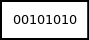
\includegraphics[scale=0.6]{img/chromosome.png}
\caption{Chromosome representation as a binary string}\label{fig:chromosome}
\end{figure}

\subsection{Fitness Function}
To fulfil the step of natural selection; the process of choosing the ``best''
members of a population, there needs to be a way of evaluating each chromosome,
such that they can be compared to one another.

The function for doing so is known as a fitness function, which typically 
returns either a single number or a list of numbers, depending on the problem.
Each chromosome can then be ranked in order of fitness and the top members of
a population can then be selected.

As the value returned from a fitness function, with be specific to the domain 
it has be used within, it is necessary to rescale the fitness value to ensure 
uniformity when genetic algorithms are applied over several different domains
at the same time. %TODO citation needed.


\subsection{Selection}
Selection simulates the ``survival of the fittest'' nature of biology. However,
it is beneficial not to keep some lesser performing members of the population
to avoid getting trapped in local optimum. Most selection algorithms will 
introduce an element of randomness into the selection to deal with this.

This report will discuss the effects of different selection algorithms in 
Section~\ref{sec:selection-algorithms}.

\subsection{Crossover}
% Talk about methods of crossover
% - Crossover point
% - Mask-based crossover
% - Other strategies (sexual, etc.) 

\subsection{Mutation}
% Talk about methods of mutation
% - Flipping bits/values

\subsection{Termination}
% Talk about termination criteria


\newpage
\section{The Effects of Selection Algorithms on GAs}
\label{sec:selection-algorithms}

The selection of the ``best'' individuals is an important step in genetic
algorithms and as such several selection algorithms have been put forward.

The simplest is to just pick the top individuals of a generation to carry on
their genes in the next generation, either through directly copying them, 
crossover or mutation.

This has its flaws and doesn't mirror the biological process of evolution. The
main flaw of this approach is that it can be beneficial to include weaker 
members of a population to avoid getting stuck in local optimum. By including
other, seemingly worse, members of a population, the effects of crossover and
mutation can overcome this problem.

Another, commonly used, technique is to use a tournament-based selection 
algorithm, which involves selecting the best member from a pool made up of
random members of the population. The size of the pool has a big effect on the
selection of individuals, and is generally inversely proportional to the
number of weaker members selected.

Tournament selection is one of the closest to biological natural selection,
and has the benefits that it is efficient, especially on parallel 
architectures.

Another popular selection algorithm is roulette-wheel selection, where the
chance a particular individual has of being selected is proportional to its
fitness. Those with a higher fitness have a higher probability of being 
selected. The equation used to calculate the probability is shown in 
equation~\ref{eq:roulette}, where $i$ is the individual in question, $f_x$ is
the fitness of individual $x$ and $N$ is the number of individuals in the 
population.

\begin{equation}
p_i = \frac{f_i}{\sum^N_{j=1}f_j}
\label{eq:roulette}
\end{equation}

There have been studies into the effects of different selection algorithms on 
genetic algorithms. Goldberg and Deb\cite{Goldberg1991Comparative} compared
four methods of selection; proportional reproduction, ranking selection,
tournament selection and the GENITOR algorithm.%TODO cite the GENITOR.

They analysed each selection scheme in terms of:

\begin{enumerate}
\item growth ratio; the expected ratio for the members of the best class to the
umber of members of the population.
\item Takeover time; the approximate number of generations it takes
to converge, this gives an idea of how long it would take before mutation,
rather than crossover, becomes the primary method for exploring the search
space. 
\item Time complexity; the standard big O measure for time complexity.
\end{enumerate}

It was found that linear ranking and binary tournament (a tournament of only
two individuals) selection had similar growth rates, but that tournament 
selection with larger pool sizes had higher growth rates, though a non-linear
ranking function can also achieve this.

Takeover times all converged in around $O(log\;n)$ generations. Most 
interestingly the time complexities had a large range, from $O(n^2)$ to $O(n)$,
with tournament selection being an $O(n)$. This is particularly interesting as
tournament selection is a very easy algorithm to make parallel, this fits in
with genetic algorithms nicely as they improve drastically from parallel 
implementation.

These results should be taken with some scepticism as they are formulated from
the pure mathematics of the selection techniques and not from running 
experiments and the authors even mention that it is only designed as a simple 
method to better understand the \textit{expected} behaviour and suggest looking
at better methods, citing the inherently noisy nature of genetic algorithms.

\subsection{Genetic Drift}
Rogers and Pr\"{u}gel-Bennett\cite{Rogers1999Genetic} defined a method of 
analysing selection schemes using genetic drift, a term borrowed from biology,
which describes the change in frequency of an allele (gene variation) through
random sampling of the population.

Genetic drift is a phenomenon observed in genetic algorithms due to the nature
of selection and, unlike analysis methods like convergence time, leads to a
exact analytical solution. Though previous attempts to calculate genetic drift
were often approximations or difficult to generalise to other cases, according
to the authors.

In genetic algorithms, genetic drift is a measure of the change in fitness
variation within a population and is worked out using probabilistic analysis of
the selection scheme. The inherent problem with this is that genetic algorithms
are a form of subsymbolic learning, which is very difficult to apply 
probabilistic methods to, due to the randomness used within them.

The authors attempt to deal this by using results from experiments averaged 
over 100,000 runs. Again though, a lot will depend on the nature of the 
problem, the representation of chromosomes and even the way in which the
selection scheme is implemented. Like with the work of Goldberg and Deb, this 
only provides an indication of the performance of a selection scheme, rather
than a full view. It does, however, seem to give some useful insights into 
different selection schemes and may help rule out less useful selection 
schemes.




\newpage
\section{Code Example}
A simple python implementation is shown in figure~\ref{lst:ga.py}.

\lstinputlisting[language=python, 
                 caption=A Python implementation of a simple Genetic 
                         Algorithm, 
                 label=lst:ga.py]{code/ga.py}
\lstinputlisting[language=python, 
                 caption=The Graph Code for listing~\ref{lst:ga.py}, 
                 label=lst:graph.py]{code/graph.py}


\bibliographystyle{plain}
\bibliography{citations}
\end{document}
